\documentclass[a4paper]{article}

\title{Architectural Design
\\COS 301 Buzz Project
\\Group 2A
\\Version 1.0}

\author{Toluwanimi Adegbenro
\\Elzahn Botha 13033922
\\Carla de Beer 95151835
\\Sboniso Masilela 10416260
\\Mandla Mhlongo 29630135
\\Isabel Nel 13070305
\\Ndivhuwo Nthambeleni 10001183
\\Lutfiyya Razak 10198408
\\
\\
\textit{https://github.com/Isabel01/COS-301-2a-Round-2}
\\
\\ University of Pretoria}

\date{11 March 2015}

% Need to compile using XeLATeX to avoid default font
\usepackage{fontspec}
\setmainfont{Arial}
% Graphics settings for .eps files
\usepackage{graphicx}
\usepackage{epstopdf}
\DeclareGraphicsExtensions{.eps}
\usepackage{float}

\begin{document}

\maketitle
% No page number to cover page
\pagenumbering{gobble}
\newpage
% start page numbering
\pagenumbering{arabic}

% Generate Table of Contents

\tableofcontents
\newpage

\section{Introduction}

\section{Architecture Requirements}

\subsection{Architectural scope}

\subsection{Quality Requirements}

\subsection{Integration and Access Channel Requirements}

\subsection{Architectural Constraints}

\section{Architectural Patterns or Styles}
An architectural pattern can be defined as a set of principles that shape an application, promote partitioning of services and reuse of code. There are a number of different patterns out there that are used for various reasons, below are some patterns we looked at to decide which ones to use;
\begin{itemize}
			\item Client/Server pattern which separates a system into two applications. Client sends requests to server and server responds to client with relevant information.
			\item Service Oriented Architecture (SOA) enables application functionality to be provided as a set of services.
			\item MVC which separates an application into View, controller and model modules.
			\item Object oriented pattern divides application into separate self-sufficient objects containing data only relevant to that object.
			\item Component-based architecture pattern focuses on the decomposition of the design into individual functional components, providing a higher level of abstraction than the OO pattern.(Microsoft Developer Network, n.d) \\[1em]
\end{itemize}
The Buzz system could consider the use of combined architectural patterns to achieve effective separation of concerns by using the Service Oriented Architecture (SOA) in which the services can be developed using a layered pattern coupled with the MVC pattern. 
The decision to use the combination of these patterns is due to the fact that the Buzz system is complex and needs to be broken down into simpler services that can be worked on separately by different teams, this will ensure responsibility localization and also improve maintainability of each sub-system. 

The services can be spread out in the following layers:
\begin{itemize}
			\item Presentation (Web Application) – Responsible for providing an interface in which users will be able to interact with the Buzz system. This will be called the BuzzWeb for the fact that it will be web based since an Android application is outside the scope of the mini project. This layer is the equivalent of the View in the MVC pattern.
			\item Web Services – This layer will be responsible for providing the services that are needed by the presentation to function, all services in the BuzzSpaces and BuzzThreads modules will be encapsulated in the web services. This forms part of the control in the MVC architecture.
			\item Business Logic – The business logic will be responsible for providing a channel to store and retrieve data from the buzz resources contained in the persistence layer. This is under the model in the MVC architecture.
			\item Persistence layer – This will include all resources that the buzz system will use, including databases and the CS dataset adapter which contains modules, students and lectures information. This is under the model in the MVC architecture.  \\[1em]
\end{itemize}

Below is a diagram to illustrate how the layers will be connected:
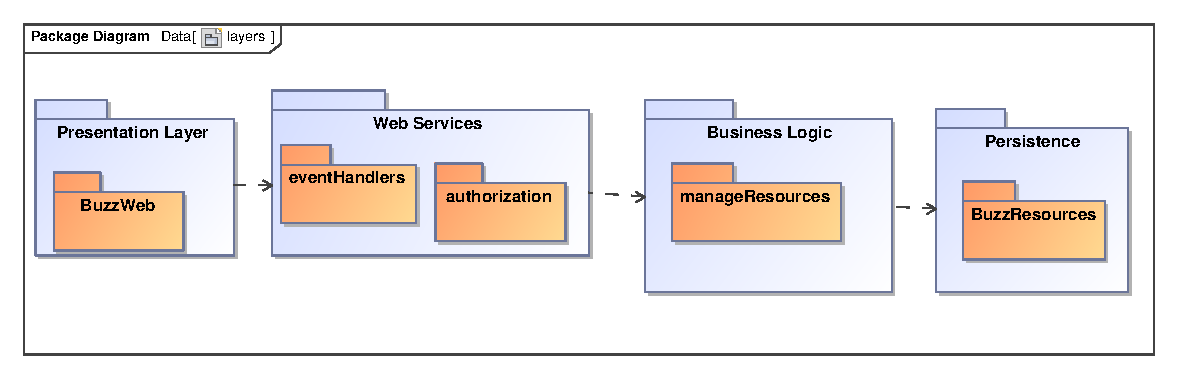
\epsfig{file=layers.eps,width=17cm}

From an MVC perspective:
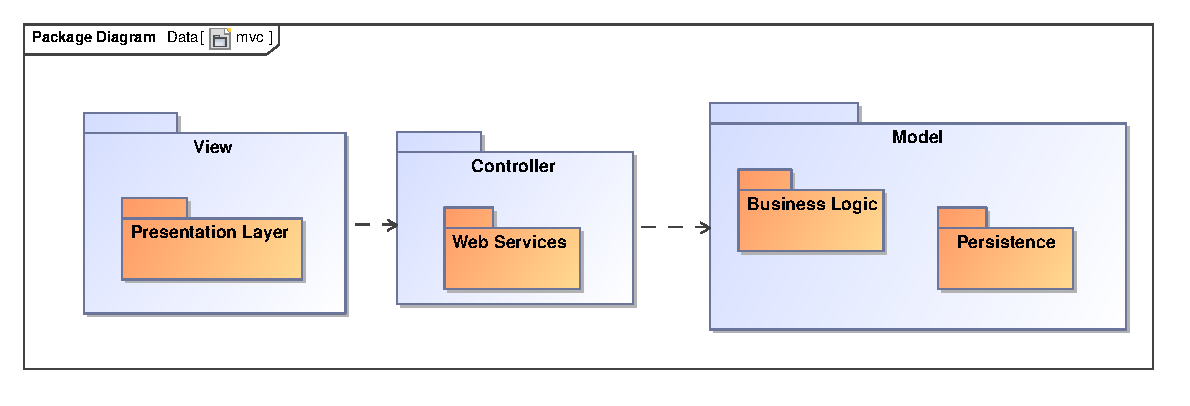
\epsfig{file=mvc.eps,width=17cm}

The integration between these layers will be in the form of APIs that each layer will provide to the layer directly above it.

Using the Layered pattern will improve on the following non-functional requirements:
\begin{itemize}
			\item Pluggability – different services can be tracked easily on the different layers, and can be replaced without compromising the whole system.
			\item Testability – Having different layers will make unit testing very simple since the layers are independent of each other, this implies that mock objects will be used to test each layer.
			\item Maintainability – Different teams can work on the different layers independently and maintain each layer separately.
			\item Security – Having authentication on the presentation layer and authorization in the Web services will increase security because each of these will be localized in one layer, however authentication is mostly left to LDAP.   \\[1em]
\end{itemize}


\section{Architectural Tactics or Strategies}

\section{Use of Reference Architectures and Frameworks}

\section{Access and Integration Channels}

\section{Technologies}

\section{References}

\end{document}
